\chapter{Bài 6. Thực hành đo tốc độ của vật chuyển động thẳng}
\begin{center}
	\textit{(3 tiết)}
\end{center}
\section{MỤC TIÊU DẠY HỌC}
\begin{center}
	\begin{longtable}{|M{2.5cm}|L{12.5cm}|M{2cm}|}
		\hline
		\thead{Biểu hiện\\ năng lực} & \thead{Mục tiêu} & \thead{STT}\\
		\hline
		\multicolumn{3}{|c|}{\textbf{ Năng lực vật lí}}\\
		\hline
		1.1 & Mô tả được một vài phương pháp đo tốc độ thông dụng và đánh giá được ưu – nhược điểm của mỗi phương pháp đo. & 1\\
		\hline
		2.3 & Thảo luận để thiết kế phương án đo tốc độ tức thời của một vật bằng dụng cụ thực hành. & 2\\
		\hline
		2.4 & Thực hiện phương án đo tốc độ tức thời của một vật bằng dụng cụ thực hành. & 3\\
		\hline
		\multicolumn{3}{|c|}{\textbf{Năng lực chung}}\\
		\hline
		CC & Tích cực tìm tòi sáng tạo trong học tập, có ý thức vượt qua khó khăn để đạt kết quả tốt trong học tập.	&4 \\
		\hline
		GT - HT & Tích cực đóng góp ý kiến trong quá trình thảo luận, biết sử dụng ngôn ngữ kết hợp với các loại phương tiện phi ngôn ngữ đa dạng để trình bày các kết quả thảo luận nhóm & 5\\
		\hline
	\end{longtable}
\end{center}
\section{THIẾT BỊ DẠY HỌC VÀ HỌC LIỆU}
\begin{itemize}
	\item Bộ thí nghiệm về chuyển động thằng đều.
	\item SGK;
\end{itemize}
\section{TIẾN TRÌNH DẠY HỌC}
\subsection{TIẾN TRÌNH}\newpage
\begin{center}
	\begin{longtable}{|L{2.75cm}|C{1.25cm}|L{5cm}|L{3.5cm}|L{4cm}|}
		\hline
		\thead{Tiến trình} & \thead{Mục\\tiêu} & \thead{Nội dung dạy học \\trọng tâm} & \thead{PP,\\ KTDH} & \thead{Phương pháp \\đánh giá}\\
		\hline
		\textbf{Hoạt động 1:} Tìm hiểu một số phương pháp đo tốc độ &1, 4  &Các phương pháp đo tốc độ thông dụng  & PPDH: Dạy học hợp tác\newline KTDH: Chia sẻ nhóm đôi & GV đánh giá dựa trên câu trả lời của HS.\newline
		PP đánh giá: quan sát, nghe.  \\
		\hline
		\textbf{Hoạt động 2:} Thiết kế phương án thí nghiệm đo tốc độ tức thời từ bộ dụng cụ thí nghiệm về chuyển động thẳng đều. & 2, 5 & Thiết kế phương án đo tốc độ tức thời từ các dụng cụ thí nghiệm có sẵn  & PPDH: Dạy học hợp tác & GV đánh giá dựa trên phương án thí nghiệm của các nhóm HS.\newline
		PP đánh giá: quan sát, nghe.  \\
		\hline
		\textbf{Hoạt động 3:} Thực hiện thí nghiệm đo tốc độ tức thời từ bộ dụng cụ thí nghiệm về chuyển động thẳng đều. & 3, 5 & Thực hiện thí nghiệm đo tốc độ tức thời của viên bi thép  & PPDH: Dạy học hợp tác & GV đánh giá dựa trên quá trình thực hiện thí nghiệm và bảng số liệu của các nhóm HS .\newline
		PP đánh giá: quan sát.  \\
		\hline
		\textbf{Hoạt động 4:} Báo cáo kết quả thí nghiệm. & 3, 5 & Xử lý kết quả thí nghiệm và viết bài thu hoạch  & PPDH: Dạy học hợp tác & GV đánh giá dựa trên bài báo cáo kết quả thí nghiệm của học sinh. \newline
		PP đánh giá: Đánh giá theo Rubric.  \\
		\hline
	\end{longtable}
\end{center}
\subsection{CÁC HOẠT ĐỘNG HỌC}
% ==========================================================================================
\hoatdong
{Tìm hiểu một số phương pháp đo tốc độ
}
{HS mô tả được một vài phương pháp đo tốc độ thông dụng và đánh giá được ưu – nhược điểm của mỗi phương pháp đo.
}
{Kết quả trả lời của HS cho các câu hỏi gợi mở của GV.
}
{\textit{\underline{* GV chuyển giao nhiệm vụ học tập}}
	\begin{itemize}[label=-]
		\item GV dẫn dắt đi vào bài học: \textit{"Ở bài 5 các em đã được học về tốc độ trung bình, tốc độ tức thời của vật chuyển động. Ở lớp 7 các em đã biết cách đo tốc độ bằng đồng hồ bấm giây. Hôm nay chúng ta sẽ học cách đo tốc độ thông qua các thiết bị đo thời gian chuyển động chính xác hơn, đặc biệt là với các chuyển động nhanh."}
		\item GV yêu cầu HS thực hiện thảo luận theo nhóm đôi để trả lời câu Thảo luận 3  SGK CTST trang 38: \textit{Quan sát Hình 6.3, tìm hiểu và trình bày phương pháp đo tốc độ trung bình và tốc độ tức thời dựa vào những thiết bị trên. Đánh giá ưu và nhược điểm của mỗi phương pháp đo.}
		\begin{center}
			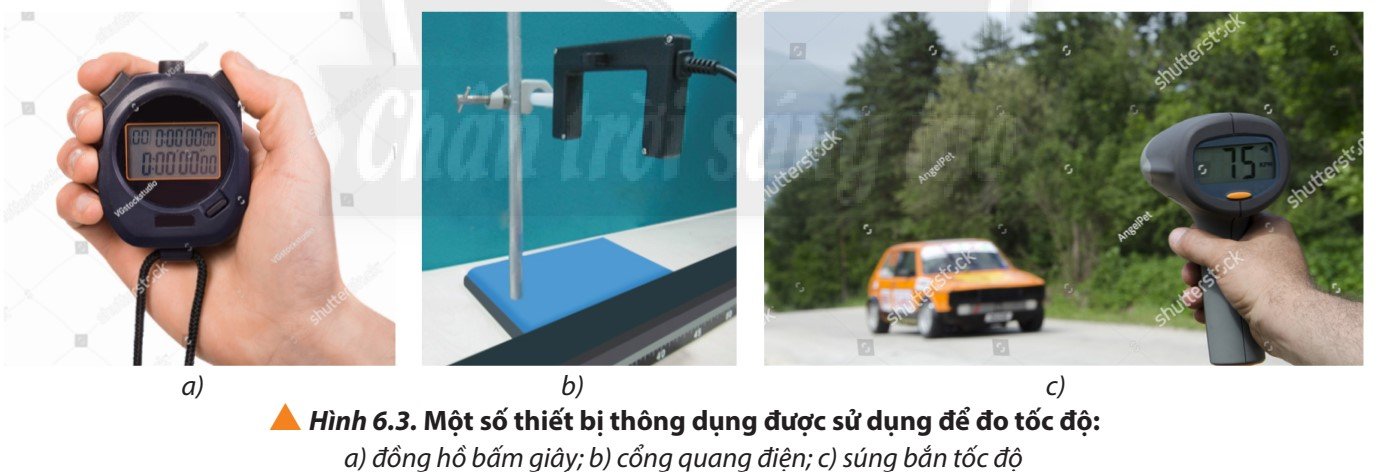
\includegraphics[scale=0.6]{figs/G10-BAI6-1}
		\end{center}
	\end{itemize}
	\textit{\underline{* HS thực hiện nhiệm vụ học tập}}\\
	HS nghiên cứu SGK, thảo luận theo nhóm và ghi câu trả lời vào giấy.\\
	\textit{\underline{* HS báo cáo kết quả nhiệm vụ học tập}}\\
	GV mời đại diện 2 nhóm HS báo cáo kết quả thảo luận nhóm. \\
	Cả lớp lắng nghe, nhận xét và đặt câu hỏi.\\
	GV chỉnh lí, hợp thức hóa kiến thức.\\
	\textbf{\textit{Gợi ý trả lời câu Thảo luận 3:}}
	\begin{itemize}
		\item Đồng hồ bấm giây: Tốc độ trung bình của vật được đo thông qua quãng đưởng vật đi được trong khoảng thời gian hiển thị trên đồng hồ.
		\item Cổng quang điện: Có thể xác định được tốc độ tức thời hoặc tốc độ trung binh của vật. Tuỳ vào cách bố trí thí nghiệm mà ta có thể xác định được giá trị tốc độ tức thời hay tốc độ trung bình tương ứng.
		\item Súng bắn tốc độ: Đối với máy bắn tốc độ sử dụng sóng âm. Phương pháp đo tốc độ dựa trên sự chênh lệch tần số sóng phát ra và sóng phản xạ quay về máy trong khoảng thời gian ngắn (đến nano giây) để đo tốc dộ tức thời của phương tiện.
	\end{itemize}
	Ưu và nhược điểm của mỗi phương pháp đo: GV có thể gợi ý cho HS nghiên cứu SGK trang 38, 39.
}
% ==========================================================================================
\hoatdong
{ Thiết kế phương án thí nghiệm đo tốc độ tức thời từ bộ dụng cụ thí nghiệm về chuyển động thẳng đều	
}
{HS thảo luận để thiết kế phương án đo tốc độ tức thời của một vật bằng dụng cụ thực hành.
	}
{Phương án thí nghiệm đo tốc độ tức thời của các nhóm HS.
}
{\textit{\underline{* GV chuyển giao nhiệm vụ học tập}}\\
	\begin{itemize}[label=-]
		\item 	GV hướng dẫn HS sử dụng thước kẹp để đo đường kính viên bi:
		\begin{center}
			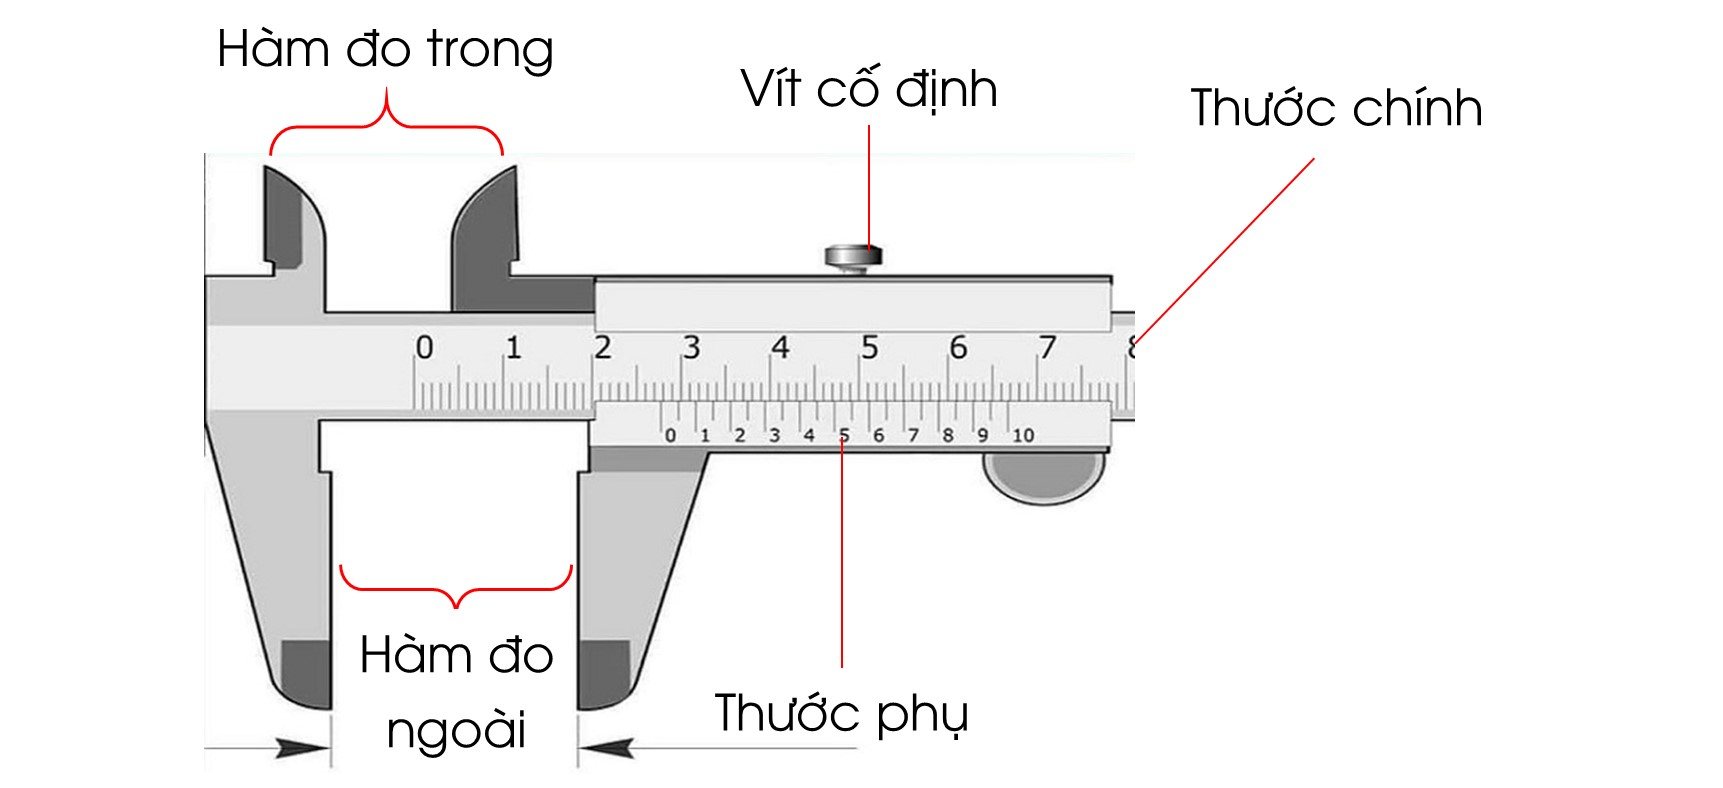
\includegraphics[scale=0.35]{figs/G10-BAI6-2}
		\end{center}
		Giá trị đo trên thước kẹp: \textbf{phần nguyên} và \textbf{phần thập phân}
		\begin{itemize}[label=$\bullet$]
			\item \textbf{Phần nguyên}: Nếu vạch 0 trên thước phụ nằm giữa hai vạch chia trên thước chính thì lấy giá trị vạch chia nhỏ hơn
			\item \textbf{Phần thập phân}: Vạch thứ $N$ trên thước phụ trùng với vạch bất kì trên thước chính thì giá trị phần thập phân được tính bằng $N\times \text{ĐCNN}$.
		\end{itemize}
		GV mời HS đọc giá trị đo trong ví dụ sau:
		\begin{center}
			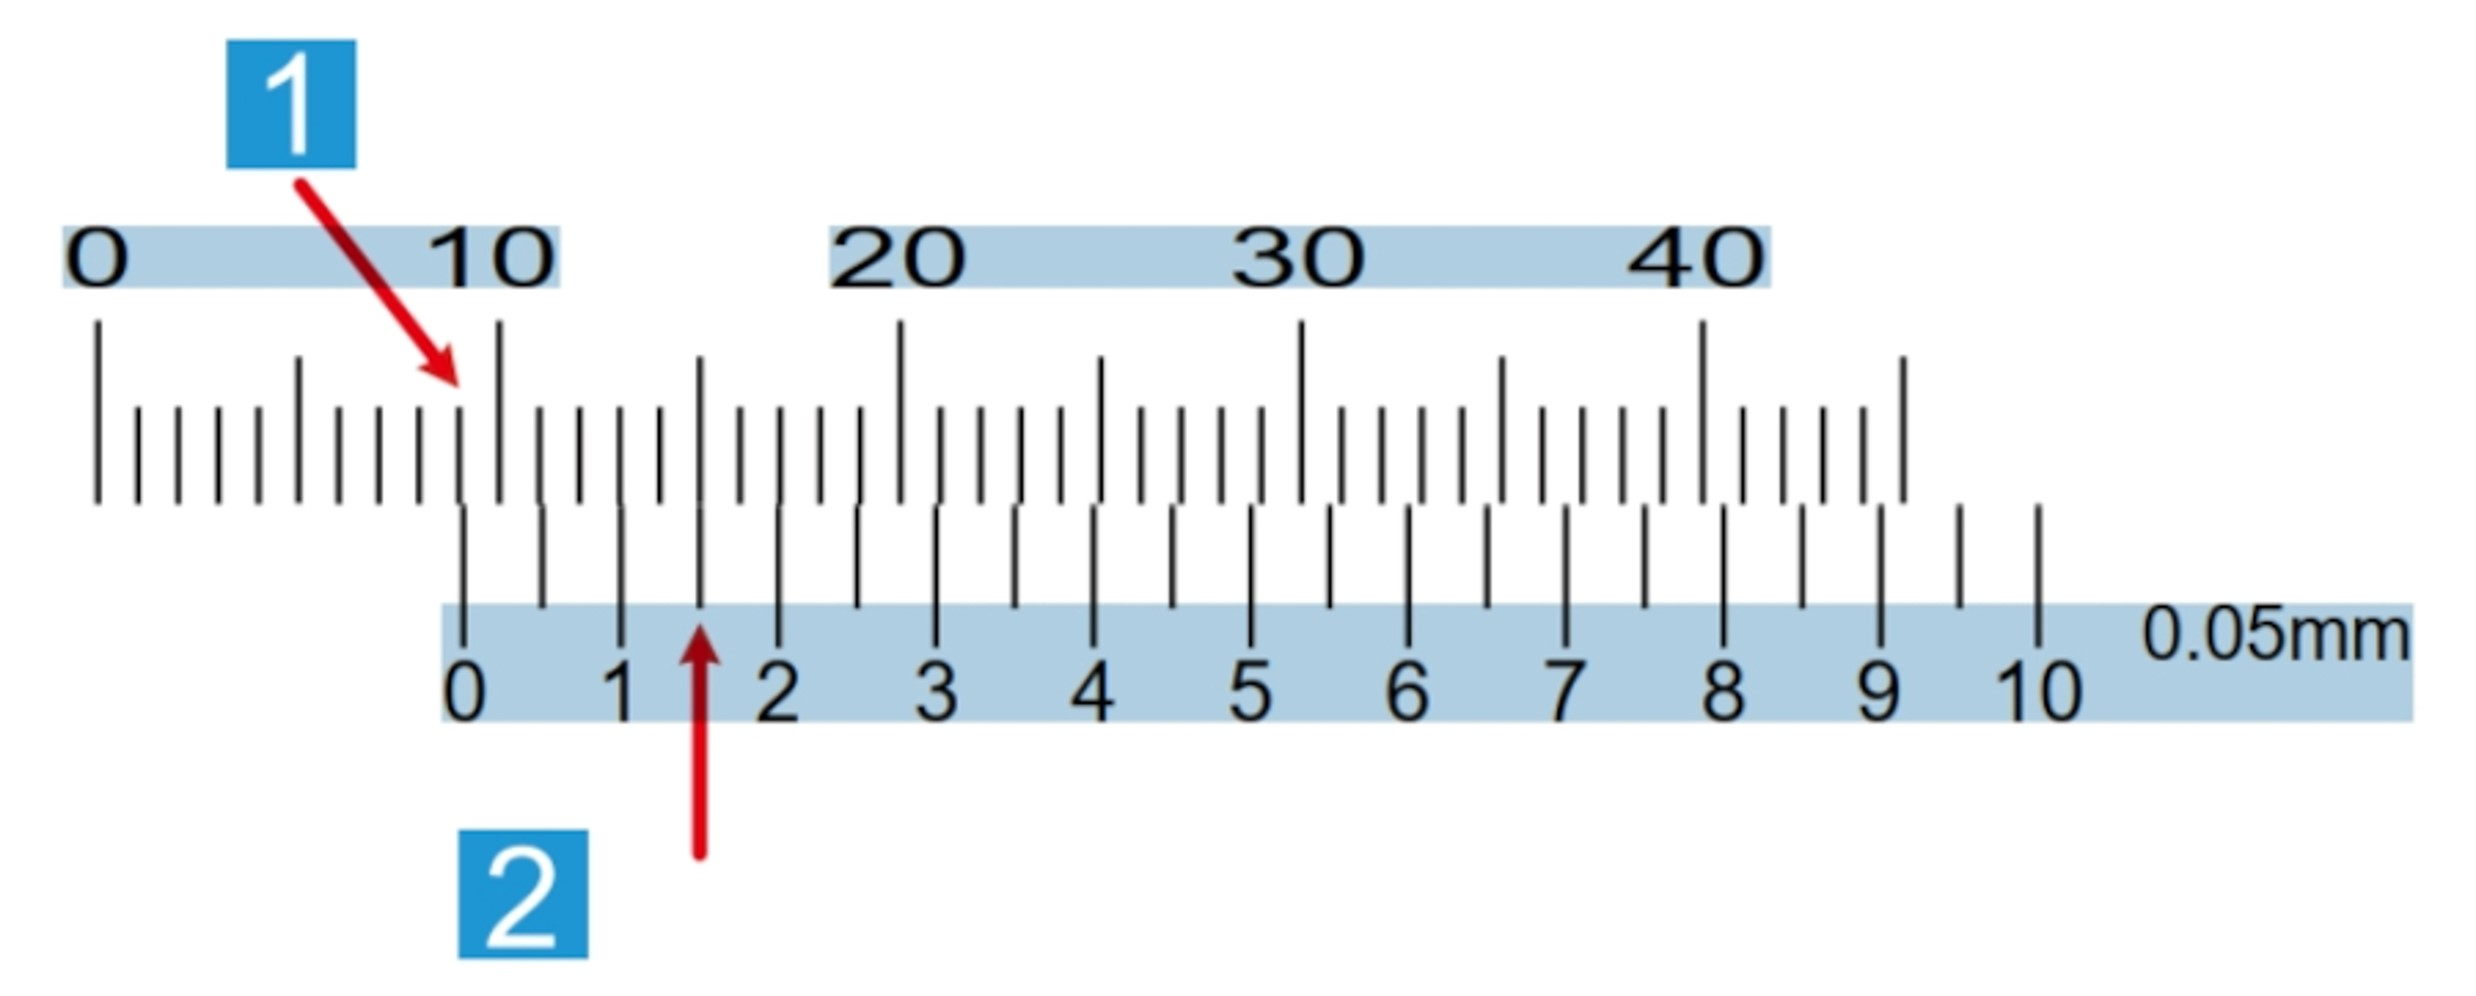
\includegraphics[scale=0.4]{figs/G10-BAI6-3}
		\end{center}
		\item 	GV giới thiệu cho HS đồng hồ đo thời gian hiện số.
		\begin{center}
			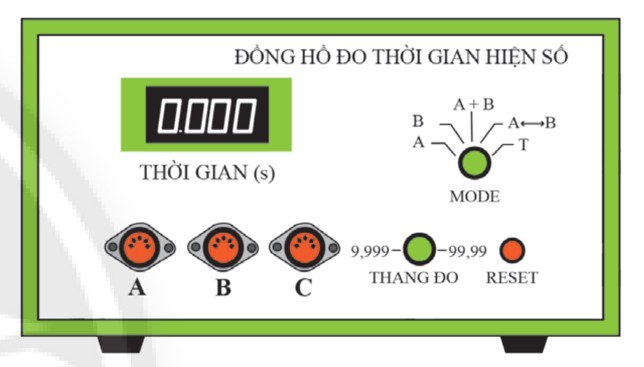
\includegraphics[scale=0.4]{figs/G10-BAI6-4}
		\end{center} 
		GV yêu cầu HS đọc phần sử dụng thiết bị đồng hồ đo thời gian hiện số trong phần chú ý SGK và trả lời các câu hỏi sau:
		\begin{itemize}[label=$\bullet$]
			\item \textbf{Câu hỏi 1:} Trên đồng hồ đo thời gian hiện số có mấy thang đo và ý nghĩa của mỗi thang đo là gì?
			\item \textbf{Câu hỏi 2:} Em hãy cho biết chức năng của các MODE  A, B, A+B, A$\leftrightarrow$B trên đồng hồ.
		\end{itemize} 
		\item GV chia lớp thành 8 nhóm. GV giới thiệu bộ dụng cụ thực hành về chuyển động. GV yêu cầu các nhóm dựa vào các dụng cụ thí nghiệm có sẵn, thảo luận nhóm để thiết kế phương án thí nghiệm đo tốc độ tức thời của viên bi thép.
	\end{itemize}
	\textit{\underline{* HS thực hiện nhiệm vụ học tập}}
	\begin{itemize}[label=-]
		\item HS chú ý lắng nghe và tích cực trả lời các câu hỏi gợi ý của GV.
		\item HS thảo luận theo nhóm được phân công để xây dựng phương án thí nghiệm đo tốc độ tức thời của viên bi thép.
	\end{itemize}
	\textit{\underline{* HS báo cáo kết quả nhiệm vụ học tập}}
	\begin{itemize}[label=-]
		\item GV mời 1 HS bất kì đọc số đo của thước kẹp trong ví dụ.\\
		\textbf{Kết quả đo trên thước kẹp:} $\SI{9.15}{\milli\meter}$.
		\item GV lần lượt đặt câu hỏi và mời HS trả lời câu hỏi 1, câu hỏi 2.\\
		\textbf{Đáp án câu hỏi:}
		\begin{itemize}[label=$\bullet$]
			\item \textbf{Câu hỏi 1}: Trên đồng hồ đo thời gian hiện số có hai thang đo $\SI{9.999}{}$ (đo thời gian chính xác đến chữ số hàng phần nghìn) và $\SI{99.99}{}$ (đo thời gian chính xác đến chữ số hàng phần trăm).
			\item \textbf{Câu hỏi 2}: Chức năng của các MODE trên đồng hồ đo thời gian hiện số:
			\begin{itemize}[label=\checkmark]
				\item MODE A hoặc MODE B: Để đo thời gian vật chắn công quang điện A hoặc cổng quang điện B.
				\item MODE A + B: đo tổng thời gian vật chắn cổng quang điện A và cổng quang điện B.
				\item MODE A$\leftrightarrow$B: đo khoảng thời gian từ lúc vật chắn công quang điện A đến thời điểm vật chắn cổng quang điện B.			
			\end{itemize}
		\end{itemize}
		\item Sau thời gian quy định, đại diện các nhóm trình bày phần thảo luận của nhóm trước lớp về phương án thí nghiệm đo tốc độ tức thời của viên bi thép. Các nhóm HS góp ý, nhận xét cho nhóm bạn.
		\item GV nhận xét và thống nhất phương án thí nghiệm với lớp.
	\end{itemize}
}
% ==========================================================================================
\hoatdong
{Thực hiện thí nghiệm đo tốc độ tức thời của viên bi
}
{HS thực hiện được phương án thí nghiệm đo tốc độ tức thời của viên bi.
}
{Bảng số liệu thí nghiệm của các nhóm HS.
}
{\textit{\underline{* GV chuyển giao nhiệm vụ học tập}}
	\begin{itemize}[label=-]
		\item GV kiểm tra thao tác lắp ráp dụng cụ thí nghiệm của các nhóm HS. Khi các nhóm đã lắp đúng thiết bị và đảm bảo an toàn thì bật nguồn và cho các nhóm tiến hành lấy số liệu.\\
		\begin{center}
			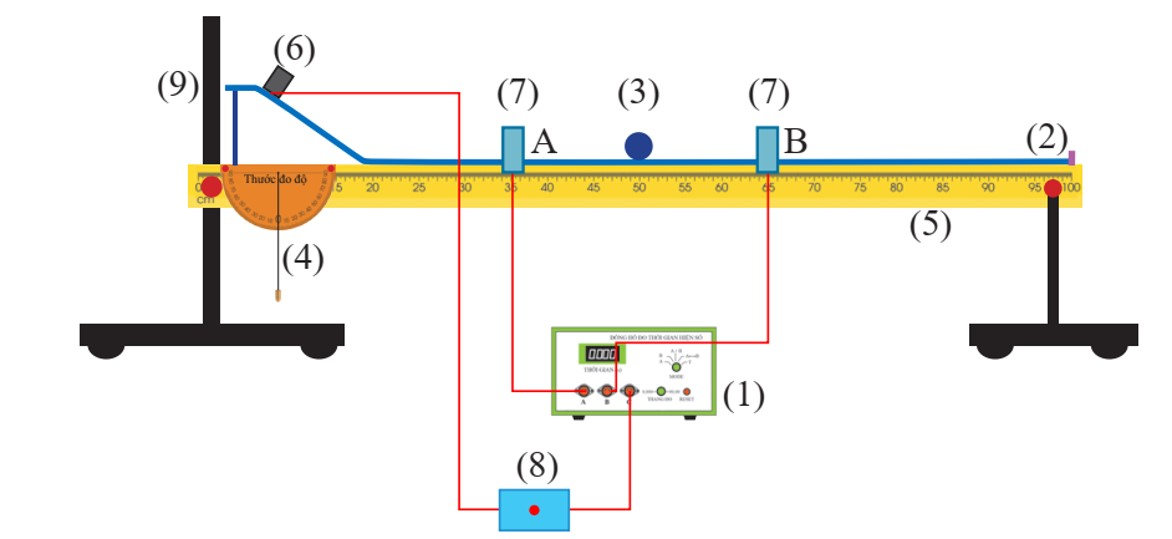
\includegraphics[scale=0.5]{figs/G10-BAI6-5}
		\end{center}
		\textbf{Sơ đồ bố trí thí nghiệm:}
		\begin{itemize}[label=$\bullet$]
			\item Đồng hồ đo thời gian hiện số có ĐCNN \SI{0.001}{\second} (1);
			\item Máng định hướng thẳng dài khoảng \SI{1}{\meter} có đoạn dốc nghiêng (độ dốc không đổi) và đoạn nằm ngang (2);
			\item Viên bi thép (3);
			\item Thước đo độ có gắn dây dọi (4);
			\item Thước thẳng ĐCNN \SI{1}{\milli\meter};
			\item Nam châm điện (6);
			\item Hai cổng quang điện (7);
			\item Công tắc điện (8);
			\item Giá đỡ (9);
			\item Thước kẹp.
		\end{itemize}
	\end{itemize}
	GV quan sát, hỗ trợ các nhóm trong quá trình thực hiện thí nghiệm.\\
	\textit{\underline{* HS thực hiện nhiệm vụ học tập}}\\
	HS tiến hành thí nghiệm nghiêm túc, trật tự, an toàn theo nhóm được phân công.\\
	\textit{\underline{* HS báo cáo kết quả nhiệm vụ học tập}}\\
	Các nhóm HS ghi nhận kết quả đo vào bảng số liệu trong phiếu học tập.
	
}
% ==========================================================================================
\hoatdong
{Xử lí kết quả thí nghiệm và viết bài thu hoạch.
}
{HS xử lí được kết quả thí nghiệm và trình bày được báo cáo thu hoạch sau thí nghiệm.	
}
{Phiếu báo cáo kết quả thí nghiệm của các nhóm HS	
}
{\textit{\underline{* GV chuyển giao nhiệm vụ học tập}}\\
	GV hướng dẫn lại cho HS các bước xử lí kết quả thí nghiệm.\\
	GV yêu cầu các nhóm HS hoàn thành bài thu hoạch tại nhà và nộp lại cho GV vào tiết học tiếp theo.\\
		\textit{\underline{* HS thực hiện nhiệm vụ học tập}}\\
		HS tích lắng nghe, đặt câu hỏi (nếu có).\\
		Các nhóm HS hoàn thành phiếu báo cáo kết quả thí nghiệm tại nhà.\\
		\textit{\underline{* HS báo cáo kết quả nhiệm vụ học tập}}\\
		Các nhóm HS nộp lại phiếu báo cáo cho GV.\\
		GV nhận xét, rút kinh nghiệm cho từng nhóm HS.
}
\section{HỒ SƠ DẠY HỌC}
\subsection{Phiếu báo cáo kết quả thực hành}\newpage
\begin{center}
	\textbf{BÁO CÁO KẾT QUẢ THỰC HÀNH THÍ NGHIỆM}\\
	\textbf{Bài 6. THỰC HÀNH ĐO TỐC ĐỘ CỦA VẬT CHUYỂN ĐỘNG THẲNG.}\\
	\textbf{\textit{(Thí nghiệm đo tốc độ tức thời của vật chuyển động)}}
\end{center}
\begin{center}
	\begin{tabular}{L{8cm}L{8cm}}
		Lớp: \dotfill&Nhóm: \dotfill
	\end{tabular}
\end{center}
\begin{center}
	\begin{tabular}{|M{1.25cm}|M{7cm}||M{1.25cm}|M{7cm}|}
		\hline
		\multicolumn{4}{M{16cm}}{\thead{Thành viên nhóm}}\\
		\hline
		\thead{STT}&\thead{Họ và tên}&\thead{STT}&\thead{Họ và tên}\\
		\hline
		1&&5&\\
		\hline
		2&&6&\\
		\hline
		3&&7&\\
		\hline
		4&&8&\\
		\hline
	\end{tabular}
\end{center}
\setcounter{section}{0}
\section{MỤC ĐÍCH THÍ NGHIỆM}
\Pointilles[2]
\section{CƠ SỞ LÍ THUYẾT}
\textit{\textbf{\underline{Câu hỏi gợi ý:}}}\\
\begin{enumerate}[label=\bfseries Câu \arabic*., leftmargin=2cm]
	\item Để đo tốc độ chuyển động của một vật ta cần đo những đại lượng nào?
	\item Dùng dụng cụ đo gì để đo các đại lượng kể trên?
	\item Phép đo tốc độ chuyển động là phép đo trực tiếp hay gián tiếp? Sai số phép đo được xác định như thế nào?
	\item Liệt kê một số phương pháp đo tốc độ. Trình bày ưu điểm và nhược điểm của từng phương pháp.
\end{enumerate}
\Pointilles[20]
\section{TIẾN HÀNH THÍ NGHIỆM}
\textit{Em hãy trình bày các bước tiến hành thí nghiệm}\\
\Pointilles[23]
\section{KẾT QUẢ THÍ NGHIỆM}
\textit{* Quy ước: 
	\begin{itemize}
		\item Giá trị trung bình của các đại lượng đo trực tiếp được lấy lớn hơn 1 bậc thập phân so với giá trị đo.
		\item Kết quả phép đo tốc độ tức thời làm tròn đến 2 chữ số sau dấu thập phân.
\end{itemize}}
\begin{center}
	\begin{tabular}{|M{1.5cm}|M{4.5cm}|M{3cm}|M{3.5cm}|M{3.5cm}|}
		\hline
		\multicolumn{5}{|M{16cm}|}{\thead{Bảng kết quả đo đường kính viên bi và \\thời gian viên bi chắn cổng quang điện.}}\\
		\hline
		\thead{Lần\\đo} & \thead{Đường kính viên bi\\
			$\xsi{d}{\left(\centi\meter\right)}$}&\thead{Sai số\\
			$\xsi{\Delta d}{\left(\centi\meter\right)}$}& \thead{Thời gian\\
			$\xsi{t}{\left(\second\right)}$}&\thead{Sai số\\
			$\xsi{\Delta t}{\left(\second\right)}$}\\
		\hline
		1&&&&\\
		\hline
		2&&&&\\
		\hline
		3&&&&\\
		\hline
		4&&&&\\
		\hline
		5&&&&\\
		\hline
		\thead{Trung\\bình}&&&&\\
		\hline
	\end{tabular}
\end{center}
\begin{tabular}{L{3.5cm}L{4cm}L{4cm}}
	Sai số dụng cụ đo:&$\Delta d_{\text{dc}}=$\dotfill&; $\Delta t_{\text{dc}}=$\dotfill
\end{tabular}\\
Kết quả phép đo đường kính viên bi:\dotfill\\
Kết quả phép đo thời gian viên bi chắn cổng quang:\dotfill\\
Kết quả phép đo tốc độ tức thời của viên bi:\dotfill\\
\Pointilles[16]
\newpage
\section{KẾT LUẬN VÀ NHẬN XÉT}
\textit{Học sinh tự kết luận về độ chính xác của kết quả phép đo trong bài thực hành, nhận xét quá trình làm thí nghiệm (những khó khăn đã gặp phải, nguyên nhân gây sai số, biện pháp khắc phục nguyên nhân gây sai số), nhận xét về kết quả làm việc nhóm (ưu điểm và nhược điểm của nhóm).}\\
\Pointilles[35]
\setcounter{subsection}{1}
\subsection{Rubric đánh giá kết quả thực hành}
	\begin{center}
	\textbf{TIÊU CHÍ ĐÁNH GIÁ THỰC HÀNH THÍ NGHIỆM}\\
	\textbf{Bài 6. THỰC HÀNH ĐO TỐC ĐỘ CỦA VẬT CHUYỂN ĐỘNG THẲNG.}
\end{center}
\begin{center}
	\begin{tabular}{L{8cm}L{8cm}}
		Lớp: \dotfill&Nhóm: \dotfill
	\end{tabular}
\end{center}
\begin{center}
	\begin{tabular}{|M{1.25cm}|M{7cm}||M{1.25cm}|M{7cm}|}
		\hline
		\multicolumn{4}{M{16cm}}{\thead{Thành viên nhóm}}\\
		\hline
		\thead{STT}&\thead{Họ và tên}&\thead{STT}&\thead{Họ và tên}\\
		\hline
		1&&5&\\
		\hline
		2&&6&\\
		\hline
		3&&7&\\
		\hline
		4&&8&\\
		\hline
	\end{tabular}
\end{center}
\textit{* Quy ước đánh giá: Ứng với mỗi chỉ số hành vi có 4 mức đánh giá, biểu hiện năng lực tốt nhất được đánh giá ở mức 3.}
\begin{center}
	\begin{longtable}{|M{1.5cm}|M{2cm}|M{1.5cm}|L{9cm}|M{1.25cm}|M{0.75cm}|}
		\hline
		\thead{Thành\\ tố}& \thead{Chỉ số\\ hành vi} &\multicolumn{2}{|M{10.5cm}|}{\thead{Tiêu chí chất lượng}}&\multicolumn{2}{|M{2.5cm}|}{\thead{Điểm}}\\
		\hline
		\multirow{12}{1.5cm}{Lập kế hoạch thí nghiệm} & \multirow{4}{2cm}{Xác định mục tiêu, cơ sở lý thuyết}  & Mức 3 & Xác định rõ ràng, chính xác, logic, nhanh chóng, không cần GV giúp đỡ. & 1.00&$\Box$\\ \cline{3-6}
		
		&  & Mức 2 & Xác định được nhưng có vài lỗi nhỏ, cần sự giúp đỡ của GV để điều chỉnh. & 0.75&$\Box$\\ \cline{3-6}
		
		&  & Mức 1 & Xác định được mục tiêu nhưng không xác định được cơ sở lý thuyết, cần hướng dẫn của GV.  & 0.50&$\Box$\\ \cline{3-6}
		
		&  & Mức 0 & Không xác định được, cần sự chỉ dẫn cụ thể của GV mới làm được.  & 0.00&$\Box$\\
		\cline{2-6}
		& \multirow{4}{2cm}{Đề xuất phương án thí nghiệm}  & Mức 3 & Đề xuất được phương án tối ưu một cách nhanh chóng, không cần sự hỗ trợ của GV.  & 0.75&$\Box$\\ \cline{3-6}
		
		&  & Mức 2 & Đề xuất được phương án có tính khả thi nhưng chưa tối ưu, cần GV sửa
		chữa, bổ sung thêm.  & 0.50&$\Box$\\ \cline{3-6}
		
		&  & Mức 1 & Đề xuất được phương án nhưng thiếu tính khả thi, cần GV định hướng.  & 0.25&$\Box$\\ \cline{3-6}
		
		&  & Mức 0 & Chưa đề xuất được phương án, cần hướng dẫn cụ thể của GV.   & 0.00&$\Box$\\
		\cline{2-6}
		& \multirow{4}{2cm}{Xây dựng tiến trình thí nghiệm}  & Mức 3 & Xác định được các dụng cụ cần thiết, xây dựng được tiến trình thí nghiệm phù hợp.  & 0.75&$\Box$\\ \cline{3-6}
		
		&  & Mức 2 & Xác định được dụng cụ cần thiết, xây dựng tiến trình dựa trên gợi ý của GV.  & 0.50&$\Box$\\ \cline{3-6}
		
		&  & Mức 1 & Xác định dụng cụ thí nghiệm chưa đầy đủ, xây dựng tiến trình dựa trên gợi ý của GV.   & 0.25&$\Box$\\ \cline{3-6}
		
		&  & Mức 0 & Chưa xác định được dụng cụ và tiến trình thí nghiệm, cần hướng dẫn cụ thể của GV.   & 0.00&$\Box$\\
		\hline
		\multirow{12}{1.5cm}{Tiến hành thí nghiệm, thu thập số liệu} & \multirow{4}{2cm}{Bố trí thí nghiệm}  & Mức 3 & Tự lắp ráp nhanh chóng, chính xác. Bố trí dụng cụ đúng sơ đồ, hợp lý về
		mặt không gian. & 1.00&$\Box$\\ \cline{3-6}
		
		&  & Mức 2 & Tự lắp ráp chính xác theo sơ đồ nhưng còn chậm và cần chỉnh sửa về mặt không gian.  & 0.75&$\Box$\\ \cline{3-6}
		
		&  & Mức 1 & Lắp ráp, bố trí theo hướng dẫn của GV nhưng còn vụng về.   & 0.50&$\Box$\\ \cline{3-6}
		
		&  & Mức 0 & Không tự lắp ráp được, GV phải làm mẫu.   & 0.00&$\Box$\\
		\cline{2-6}
		& \multirow{4}{2cm}{Thao tác thí nghiệm}  & Mức 3 & Tự lựa chọn đúng thang đo, điều chỉnh dụng cụ một cách chính xác, nhanh chóng.   & 1.00&$\Box$\\ \cline{3-6}
		
		&  & Mức 2 & Tự lựa chọn đúng thang đo, điều chỉnh được dụng cụ nhưng còn chậm.   & 0.75&$\Box$\\ \cline{3-6}
		
		&  & Mức 1 & Lựa chọn được thang đo, điều chỉnh được dụng cụ dưới sự hướng dẫn của GV.   & 0.50&$\Box$\\ \cline{3-6}
		
		&  & Mức 0 & Không biết cách thao tác.    & 0.00&$\Box$\\
		\cline{2-6}
		& \multirow{4}{2cm}{Quan sát, đọc và ghi kết quả}  & Mức 3 & Quan sát và đọc, ghi kết quả một cách nhanh chóng, chính xác.   & 1.00&$\Box$\\ \cline{3-6}
		
		&  & Mức 2 &  Quan sát và đọc, ghi được kết quả nhưng còn chậm.   & 0.75&$\Box$\\ \cline{3-6}
		
		&  & Mức 1 & Quan sát và đọc, ghi được kết quả dưới sự hướng dẫn của GV.    & 0.50&$\Box$\\ \cline{3-6}
		
		&  & Mức 0 &  Hoàn toàn quan sát và đọc, ghi kết quả theo thao tác mẫu của GV.    & 0.00&$\Box$\\
		\hline
		\multirow{8}{1.5cm}{Thái độ thực hành} & \multirow{4}{2cm}{An toàn thí nghiệm}  & Mức 3 & Đảm bảo các quy tắc an toàn trong thực hành thí nghiệm, tác phong nghiêm túc, trật tự, có tinh thần tự giác trong học tập. & 0.75&$\Box$\\ \cline{3-6}
		
		&  & Mức 2 & Đảm bảo các quy tắc an toàn trong thực hành thí nghiệm, tác phong nghiêm túc, trật tự.  & 0.50&$\Box$\\ \cline{3-6}
		
		&  & Mức 1 & Đảm bảo các quy tắc an toàn trong thực hành thí nghiệm, tác phong nghiêm túc, còn gây mất trật tự trong quá trình thực hành.   & 0.25&$\Box$\\ \cline{3-6}
		
		&  & Mức 0 & Không tuân thủ các quy tắc an toàn thí nghiệm, gây mất trật tự trong giờ thực hành.   & 0.00&$\Box$\\
		\cline{2-6}
		& \multirow{4}{2cm}{Trách nhiệm và tích cực}  & Mức 3 & Có tinh thần trách nhiệm trong làm việc nhóm, $\SI{100}{\percent}$ thành viên tích cực tham gia thực hành.   & 0.75&$\Box$\\ \cline{3-6}
		
		&  & Mức 2 & Có tinh thần trách nhiệm trong làm việc nhóm, $\SI{75}{\percent}$ thành viên tích cực tham gia thực hành.   & 0.50&$\Box$\\ \cline{3-6}
		
		&  & Mức 1 & Xao lãng trong làm việc nhóm, $\SI{50}{\percent}$ thành viên tích cực tham gia thực hành.   & 0.25&$\Box$\\ \cline{3-6}
		
		&  & Mức 0 & Xao lãng trong làm việc nhóm, dưới $\SI{50}{\percent}$ thành viên tham gia thực hành.    & 0.00&$\Box$\\
		\hline
		\multirow{12}{1.5cm}{Xử lý kết quả thí nghiệm} & \multirow{4}{2cm}{Xử lý kết quả đo trực tiếp và gián tiếp}  & Mức 3 & Sử dụng công thức phù hợp, tính toán nhanh chóng, kết quả chính xác, phù hợp với số liệu thực tiễn.  & 1.25&$\Box$\\ \cline{3-6}
		
		&  & Mức 2 & Sử dụng công thức phù hợp, tính toán còn chậm, kết quả còn một vài sai sót nhỏ, phù hợp với số liệu thực tiễn.   & 1.00&$\Box$\\ \cline{3-6}
		
		&  & Mức 1 & Cần sự hướng dẫn của GV, còn nhầm lẫn trong tính toán, kết quả sai lệch so với số liệu thực tiễn.    & 0.50&$\Box$\\ \cline{3-6}
		
		&  & Mức 0 & Không tính toán được.    & 0.00&$\Box$\\
		\cline{2-6}
		& \multirow{4}{2cm}{Độ tin cậy của kết quả thí nghiệm}  & Mức 3 & Sai số tỉ đối của phép đo dưới $\SI{5}{\percent}$.   & 0.75&$\Box$\\ \cline{3-6}
		
		&  & Mức 2 & Sai số tỉ đối của phép đo dưới $\SI{10}{\percent}$.   & 0.50&$\Box$\\ \cline{3-6}
		
		&  & Mức 1 & Sai số tỉ đối của phép đo dưới $\SI{15}{\percent}$.   & 0.25&$\Box$\\ \cline{3-6}
		
		&  & Mức 0 & Không xác định được sai số tỉ đối hoặc sai số tỉ đối trên $\SI{15}{\percent}$.    & 0.00&$\Box$\\
		\cline{2-6}
		& \multirow{4}{2cm}{Kết luận, nhận xét, đánh giá}  & Mức 3 & Viết đúng kết quả phép đo, nhận xét chính xác quá trình làm thí
		nghiệm, tìm được nguyên nhân gây sai số và đề xuất được biện pháp khắc phục.   & 1.00&$\Box$\\ \cline{3-6}
		
		&  & Mức 2 &  Viết đúng kết quả phép đo, nhận xét chính xác quá trình làm thí nghiệm, tìm được nguyên nhân gây sai số nhưng không đề xuất được biện pháp khắc phục.   & 0.75&$\Box$\\ \cline{3-6}
		
		&  & Mức 1 & Viết sai kết quả đo, nhận xét được quá trình làm thí
		nghiệm nhưng còn sơ sài, thiếu chính xác, không tìm được nguyên nhân gây sai số.    & 0.50&$\Box$\\ \cline{3-6}
		
		&  & Mức 0 &  Không có hoặc không thể kết luận, nhận xét.    & 0.00&$\Box$\\
		\hline
		\hline
		\multicolumn{6}{|M{16cm}|}{\thead{TỔNG ĐIỂM: \hspace{1cm} /10.00  }}\\
		\hline
		\hline
	\end{longtable}
\end{center}

